% Drawing 43/04-8 -- folder 43, batch 04, archive page 62 (PDF page 63).
% Transcription: au-dessous, à gauche, trois segments fléchés consécutifs sur une même ligne, légendés $c$, $c'$, $c''$.
% Kind: three consecutive arrows c, c', c''. Method 2 (schematic redraw from the facsimile). Status: ok.
% Notes: Ink. Three short arrows end to end on one line, each pointing right, the middle one heavy, with the letters c, c', c'' above them. The « A_c » to their right is text. Redrawn 2026-11-12 (issue 128): to check again.
% Coordinates: 1 unit = 1 mm = 1/100 of the crop width, y downwards as on the crop (bbox in page fractions: [0.14, 0.755, 0.5, 0.83]).
% Redrawn by Claude (claude-fable-5-2), issue #128, 2026-11-12; not checked by a human; not compiled (no TeX in the session).
% Rights: reproduces part of the work -- behind RENDER_TRANSCRIPTS, never published by itself.
\documentclass[tikz,border=3pt]{standalone}
\usepackage{amsmath,amssymb}
\usetikzlibrary{patterns,arrows.meta}
\tikzset{pencil/.style={black!45}, struck/.style={black!35}, mpt/.style={circle,draw,inner sep=1.3pt}, pt/.style={circle,fill,inner sep=0.9pt}, opt/.style={circle,draw,fill=white,inner sep=1.1pt}, Rd/.style={red!75!black}, Gn/.style={green!45!black}, Br/.style={brown!70!black}}
\begin{document}
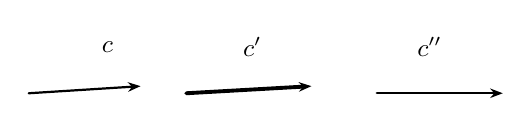
\begin{tikzpicture}[x=1mm,y=-1mm,line cap=round,line join=round,font=\small]
\draw[thick,-{Stealth[length=1.6mm]}] (25.8,16.7) -- (40,15.8);
\draw[line width=1.4pt,-{Stealth[length=1.6mm]}] (45.8,16.7) -- (61.7,15.8);
\draw[thick,-{Stealth[length=1.6mm]}] (70,16.7) -- (86,16.7);
\node at (35.8,10.8) {$c$};
\node at (54.2,10.8) {$c'$};
\node at (76.7,10.8) {$c''$};
\end{tikzpicture}
\end{document}
